\RequirePackage{amsthm} %https://tex.stackexchange.com/questions/687324/unknown-theoremstyle-warning-with-springer-nature-template
\documentclass[sn-mathphys-num,icol]{sn-jnl}
%\documentclass[sn-mathphys-num,iicol]{jnl}

%\usepackage{sn-jnl.sty}
\usepackage[pscoord]{eso-pic}% The zero point of the coordinate systemis the lower left corner of the page (the default).

\usepackage[absolute,overlay]{textpos}
\usepackage[dvipsnames]{xcolor}
\usepackage{tikz}
\usepackage{graphicx}% \usepackage{multirow}% \usepackage{cuted}
\usepackage{amsmath,amssymb,amsfonts}%
\usepackage{multicol}
\usepackage{multirow}
\usepackage{amsthm}%
\usepackage{gensymb}
\usepackage{physics}
\usepackage[locale=US]{siunitx}
\usepackage{mathrsfs}%
\usepackage[title]{appendix}%
\usepackage{xcolor}%
\usepackage{textcomp}%
\usepackage{manyfoot}%
\usepackage{booktabs}%
\usepackage{algorithm}%
\usepackage{algorithmicx}%
\usepackage{algpseudocode}%
\usepackage{listings}%
\usepackage{newtxmath}%
\usepackage{yfonts}
\usepackage{braket}
\usepackage{dsfont}
\usepackage{subcaption}
\usepackage[tiny]{titlesec}%
\usepackage[american]{babel}
\usepackage{cleveref}

\usetikzlibrary{arrows.meta, positioning, shapes.geometric, decorations.markings}

\theoremstyle{thmstyleone}
\newtheorem{theorem}{Theorem}
\newtheorem{proposition}[theorem]{Proposition}

\theoremstyle{thmstyletwo}
\newtheorem{remark}{Remark}

\theoremstyle{thmstylethree}
\newtheorem{definition}{Definition}

\raggedbottom

\newcommand{\td}{\text{d}}

\titleformat{\subsection}{}{\thesubsection}{1em}{\itshape}
\titleformat{\subsubsection}{}{\thesubsubsection}{1em}{\itshape}

\begin{document}

\title{M2.3: Transport Properties of Copper}
\author*[1]{\fnm{Dhruv} \sur{Pisharody}}\email{s36drohi@uni-bonn.de}
\author*[1]{\fnm{Ahmet} \sur{Kavruk}}\email{s37akvr@uni-bonn.de}
\author*[1]{\fnm{Angelo} \sur{Brade}}\email{s72abrad@uni-bonn.de}
\affil*[1]{Rheinische Friedrich--Wilhelms--Universität, Bonn}
\maketitle

\subsection{Model Measurements}
\subsubsection{Electric Resistivity}
To investigat the electric resistivity a current ranging from \SI{-100}{mA} to \SI{100}{mA} in \SI{20}{mA} steps is applied. The data points at ambient pressure are show in \Cref{fig:aer} and in vaccuum in \Cref{fig:vac}. As there is the possiblity of some residue current, producing a voltage, a linear function is fittet. The y-axis shift is the the extra voltage produced by the resedure current.
\begin{figure}
	\centering
	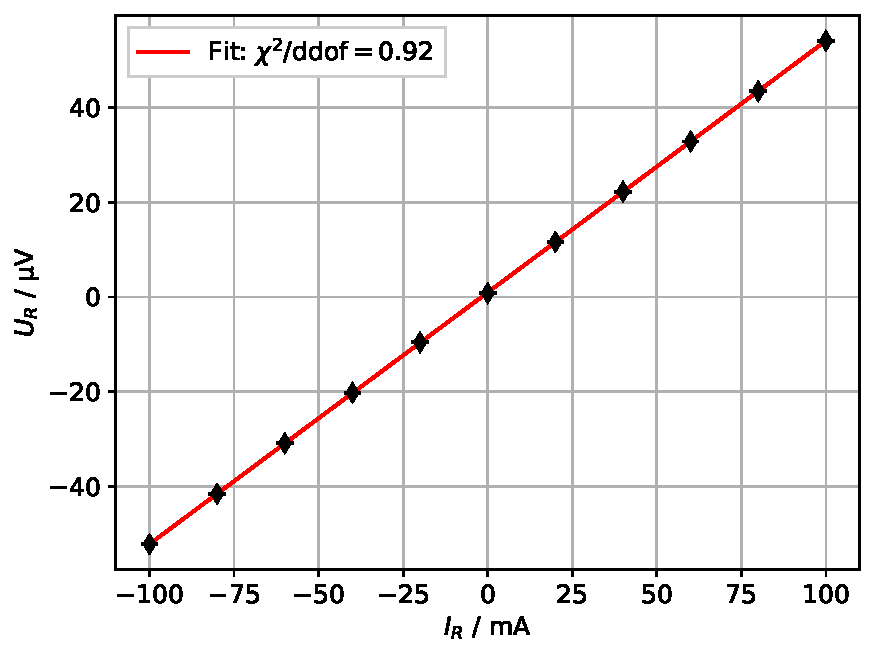
\includegraphics[width=1\textwidth]{../images/aer.pdf}
	\caption{Electric Voltage at Ambient Pressure; Fit: $U^a_\text{R}(I_\text{R})=\SI{531.53+-0.35}{\mu\Omega}\cdot I_R +\SI{9.29+-0.22}{nV}$}\label{fig:aer}.
\end{figure}
\begin{figure}
	\centering
	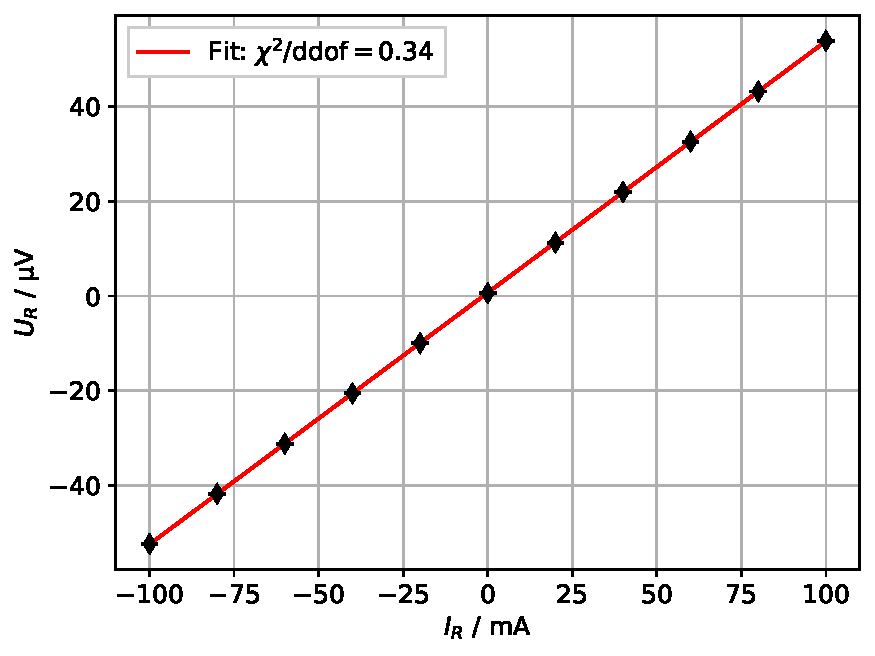
\includegraphics[width=1\textwidth]{../images/ver.pdf}
	\caption{Elecgric Voltage in a Vacuum; Fit: $U^v_\text{R}(I_\text{R})=\SI{531.11+-0.38}{\mu\Omega}\cdot I_\text{R}+\SI{7.09+-0.25}{nV}$}\label{fig:vac}
\end{figure}
Both $\chi^2/\text{ddof}$ are close to 1, so the uncertainties are reasonable.

To calculate the electrical resistivity the extra current of $U^a_0=\SI{9.29+-0.22}{nV}$ and $U^v_0=\SI{7.09+-0.25}{nV}$ respectively are subtracted from the initial current. Thus the resulting current reads as formula
\begin{align}
	\rho=\frac{A(U^a_\text{R} - U^a_0)}{I_\text{R}l_\text{R}}
\end{align}
with the distance between the two current probing contacts $l_\text{R}=\SI{48.8+-2.0}{mm}$, and the croess-sectional area $A=d\cdot b$ with $d=\SI{0.1111+-0.00015}{mm}$ and $b=\SI{15.28+-0.09}{mm}$. The resistivity is shown in \Cref{fig:aer2} and \Cref{fig:ver2}. The $\chi^2/\text{ddof}$ are notably low, which result from the fact, that the data points are nearly independent of the current $I_\text{E}$ and thus lie all on the fit function. A fit is perhaps not appropriate here and thus the concept of a fit-quality breaks down.

Within the precision of the obtained data, it can be assumed that the electric resistivity is independent of the current. The data yields the electric resistivity $\rho^a=\SI{18.46+-.26}{n\Omega m}$ for ambient pressure and $\rho^v=\SI{18.46+-.26}{n\Omega m}$ in a vacuum. As both values are in a $6.46\sigma$ interval to the literature value \SI{16.78}{n\Omega m}\cite{crc_handbook_chem_phys} at \SI{293}{K}, a systematic error is detected. This error can be caused by the contact resistance of the source contacts of the 4-point measurement.

\begin{figure}
	\centering
	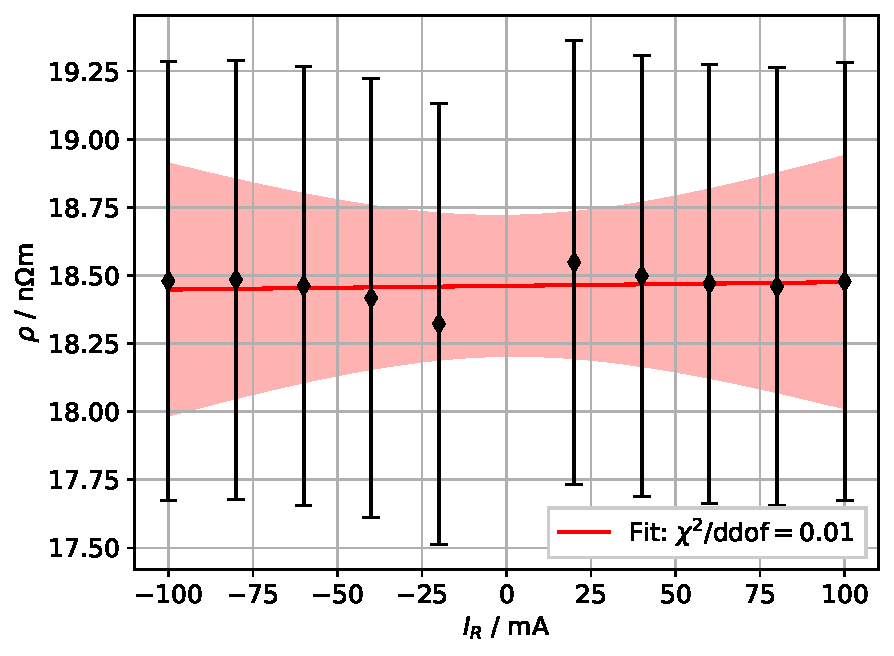
\includegraphics[width=1\textwidth]{../images/aer2.pdf}
	\caption{Electrical Resistivity at Ambient Pressure; Fit: $\rho^a(I) = \SI{.1+-3.8}{\frac{n\Omega m}{A}}\cdot I + \SI{1846+-26}{n\Omega m}$}\label{fig:aer2}
\end{figure}
\begin{figure}
	\centering
	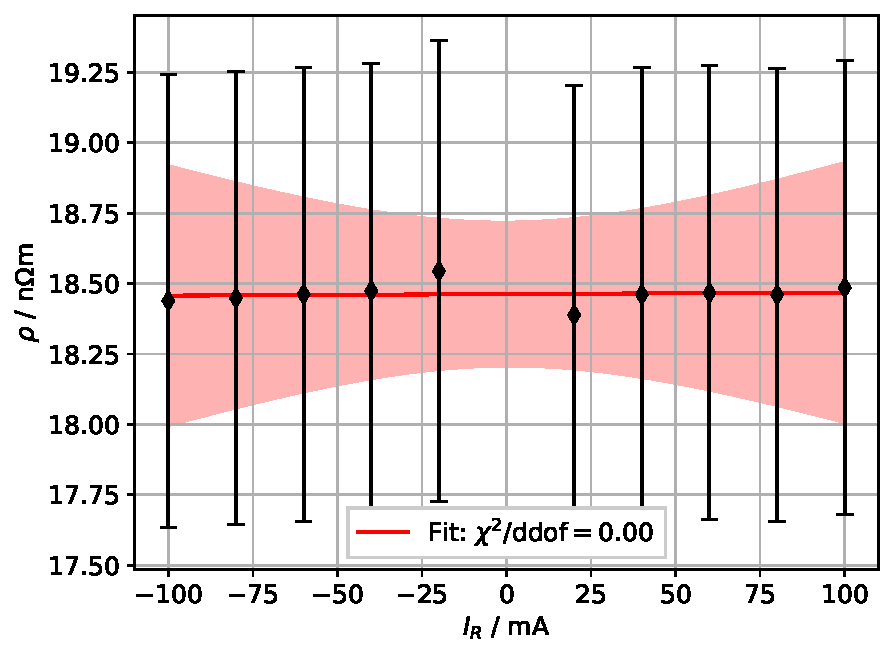
\includegraphics[width=1\textwidth]{../images/ver2.pdf}
	\caption{Electrical Resistivity in a Vacuum; Fit: $\rho^a(I) = \SI{.1+-3.8}{\frac{n\Omega m}{A}}\cdot I + \SI{18.46+-0.26}{n\Omega m}$}\label{fig:ver2}
\end{figure}
?
\subsubsection{Thermal Conductivity}
For the thermal conductivity a current ranging from \SI{0}{mA} to \SI{5}{mA} in \SI{1}{mA} steps is used for the heater. The measured thermoelectric voltages are shown in \Cref{fig:atc} and \Cref{fig:vtc}.


\begin{figure}
	\centering
	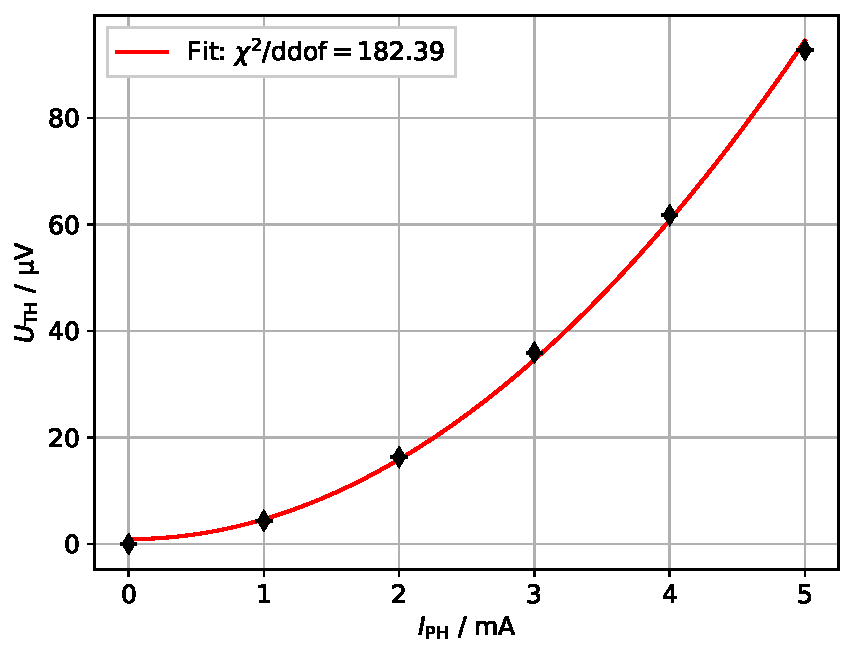
\includegraphics[width=1\textwidth]{../images/atc.pdf}
	\caption{Thermalelectric voltage at Ambient Pressure; Fit: $U_{\text{TH}}(I_\text{R})=\SI{3.7434+-0.0048}{\frac{V}{I^2}}I_{\text{PH}}^2+\SI{890+-56}{n V}$}\label{fig:atc}
\end{figure}
\begin{figure}
	\centering
	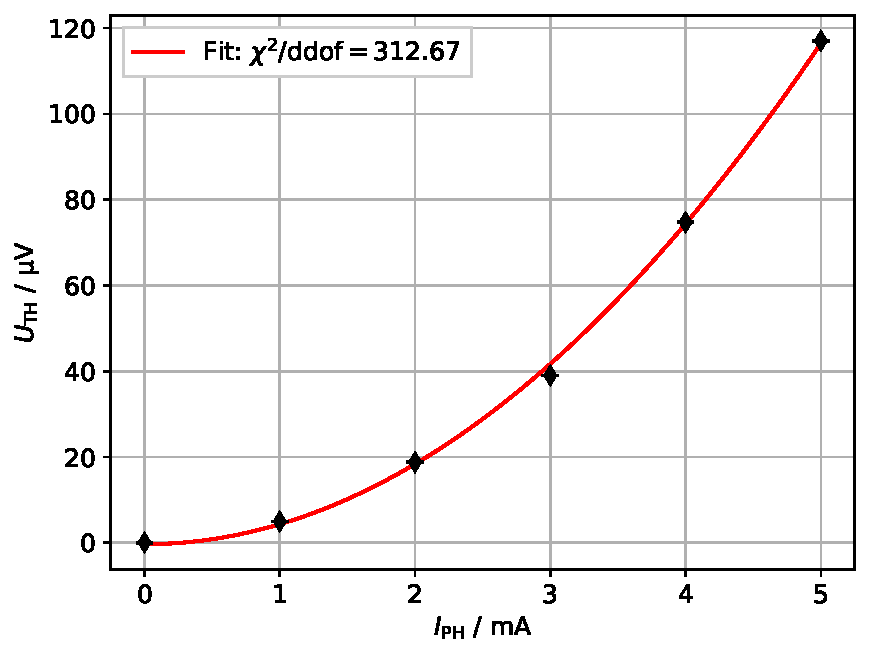
\includegraphics[width=1\textwidth]{../images/vtc.pdf}
	\caption{Thermalelectric voltage in a Vacuum; Fit: $U_{\text{TH}}(I_\text{R})=\SI{4.6703+-0.0038}{\frac{V}{I^2}}I_{\text{PH}}^2+\SI{-343+-047}{n V}$}\label{fig:vtc}
\end{figure}

Using the relation
\begin{align}
	\kappa=\frac{U_{\text{PH}}I_{\text{PH}}S(T,B)l_{\text{LE}}}{U_{\text{TE}}A}
\end{align}
with $U_{\text{PH}}=R_{\text{PH}}I_{\text{PH}}$ \Cref{fig:atc2} and \Cref{fig:vtc2} are obtained.

\begin{figure}
	\centering
	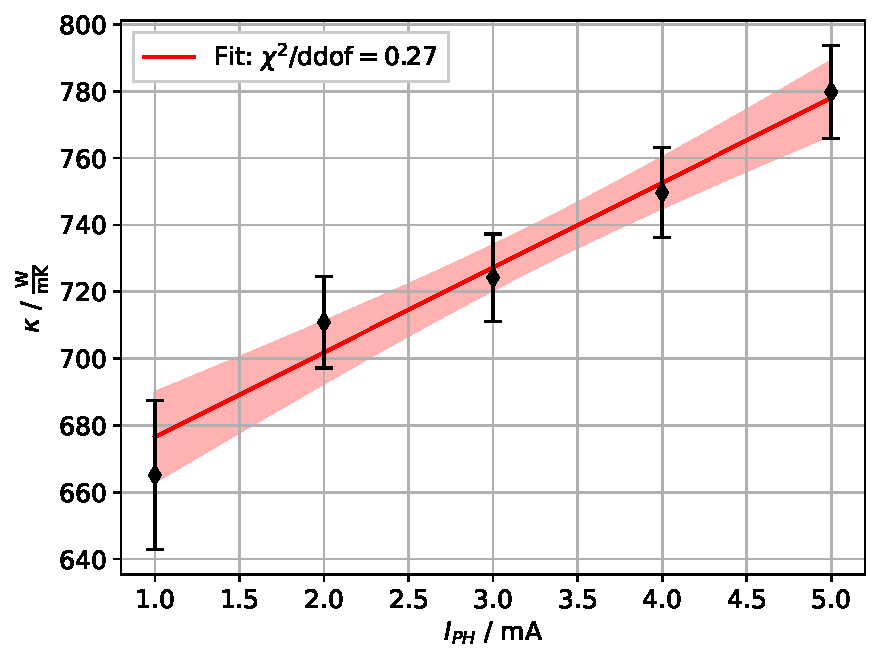
\includegraphics[width=1\textwidth]{../images/atc2.pdf}
  \caption{Thermal conductivity at ambient pressure: $\kappa(I_\text{PH})=\SI{25400.0+-5100.0}{\frac{kW}{m\cdot K\cdot A}}+\SI{651.0+-18.0}{\frac{W}{m\cdot K}}I_\text{PH}$}\label{fig:atc2}
\end{figure}
\begin{figure}
	\centering
	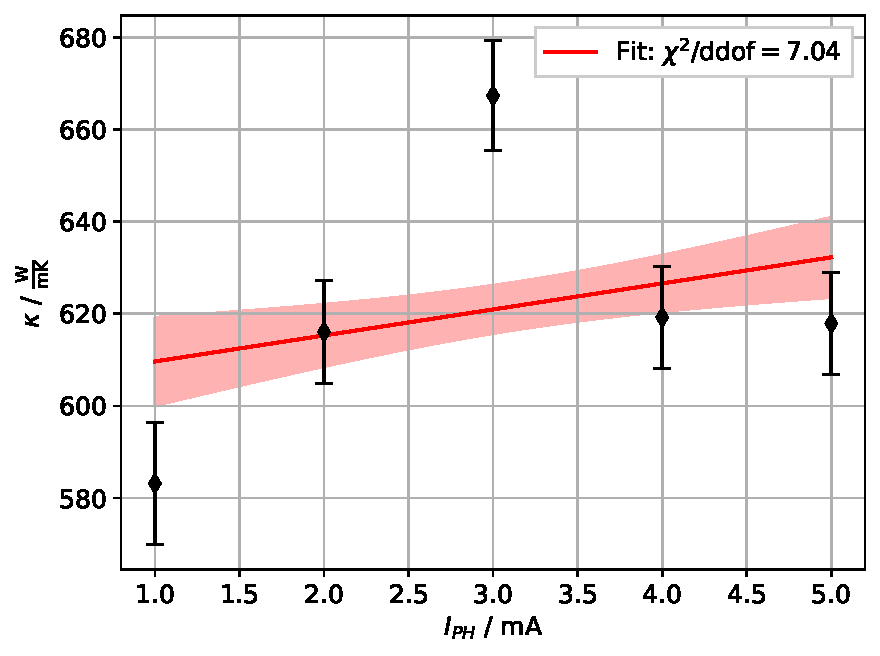
\includegraphics[width=1\textwidth]{../images/vtc2.pdf}
  \caption{Thermal conductivity in a vacuum: $\kappa(I_\text{PH})=\SI{5.6+-3.8}{\frac{kW}{m\cdot K\cdot A}}+\SI{604.0+-13.0}{\frac{W}{m\cdot K}}I_\text{PH}$}\label{fig:vtc2}
\end{figure}

Here it can be seen that the thermal conductivity is dependent on the heating current at ambient pressure. In the vacuum the dependency is largely lost. This bevhavioure stems from the air around the sample. It can transport the heat through convection, which is a process with a dependent on the temperature, i.e. the heating current. As we approach the vacuum this contribution vanishes, as reflected in the data. Inspecting the rough ranges of thermal conductivity of both figures, one sees that the values are in general larger at similar currents in the air measurement then in the vacuum measurement. This is also due to the air which helps to transport the heat, thus making the thermal conductivity larger.

Unexpected is the observation, both thermal conductivities lie above the literature value $\kappa_\text{lit}=\SI{401}{\frac{W}{mK}}$. Expected would be that the data would be below the literature value, since copper is in general very heat conductive and any building elements in the apparatus would rather be more insulating then have a higher thermal conductance. Therefore an unknown systematical error may apply.

Assuming the vacuum measurement to be independent of the heating current $I_\text{PH}$, the obtained value is with \SI{604.0+-13.0}{\frac{W}{m\cdot K}} about $15.6\sigma$ away from the literature value. This Also hints a systematical error. If the measured conductance would have been lower then the literature value, this discrepancy could have been explained by the contacts, which might be not as conducting as the copper. But as we have higher conductances, the authors can not think of a plausible explanation.

Lastly the temperature gradient is calculated via
\begin{align}
	\nabla T=\frac{\Delta T}{l_\text{TE}}=\frac{U_\text{TE}}{S(T,B)l_\text{TE}}
\end{align}
with the thermoelectric power given by $S=\SI{59}{\frac{mV}{K}}$. The values are shown in \Cref{fig:atg} and \Cref{fig:vtg}


\begin{figure}
	\centering
	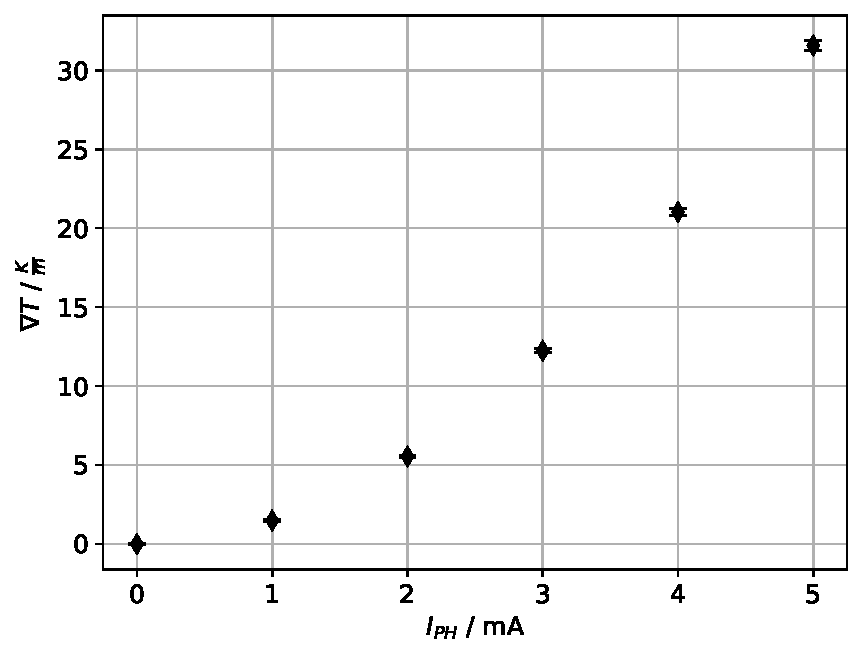
\includegraphics[width=1\textwidth]{../images/atg.pdf}
	\caption{Temperature Gradient at Ambient Pressure.}\label{fig:atg}
\end{figure}
\begin{figure}
	\centering
	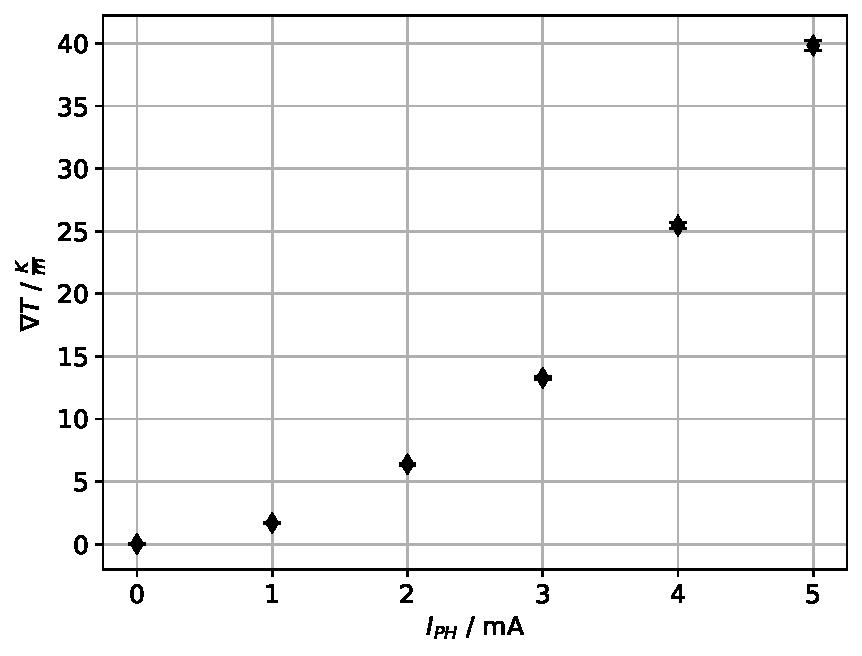
\includegraphics[width=1\textwidth]{../images/vtg.pdf}
	\caption{Temperature Gradient in a Vacuum}\label{fig:vtg}
\end{figure}

As one can see, a cubed dependency on the $I_\text{PH}$ is measured. Thus squaring the data beforehand could be a reasonable plot. But to as the square root of the temperature gradient is not commonly used, this report will keep the simple non-square root representation of the data.

This cubed behaviour is expected as the heating power is dependent on the heater current squared.

Just as discussed for the electric resistivity and as for the thermal conductivity, both measured values for $\rho$ and $\kappa$ are rather far from the literature value, but since their magnitudes are very comparable, all measured values are reasonable.

\subsection{Resistivity}
For the temperatures \SI{10}{K}, \SI{20}{K}, \SI{30}{K} and \SI{40}{K} and for the magnetic field strengths of \SI{-6}{T} to \SI{6}{T} the data is recorded with a prepared dip-stick and are controlled by a computer. These measurements run overnight and are provided to us. The resistivity is calculated as before, but now with the values
$d = \SI{0.1111 \pm 0.0015}{\milli\metre}$,
$b = \SI{2.16 \pm 0.05}{\milli\metre}$,
$l_{\mathrm{TC}} = \SI{16.2 \pm 0.5}{\milli\metre}$,
$l_{\mathrm{R}} = \SI{12.2 \pm 0.5}{\milli\metre}$,
and $R_{\mathrm{PH}} = \SI{1}{\kilo\ohm}$. The resistivity is shown in \Crefrange{fig:res0}{fig:res3}.
\begin{figure}
	\centering
	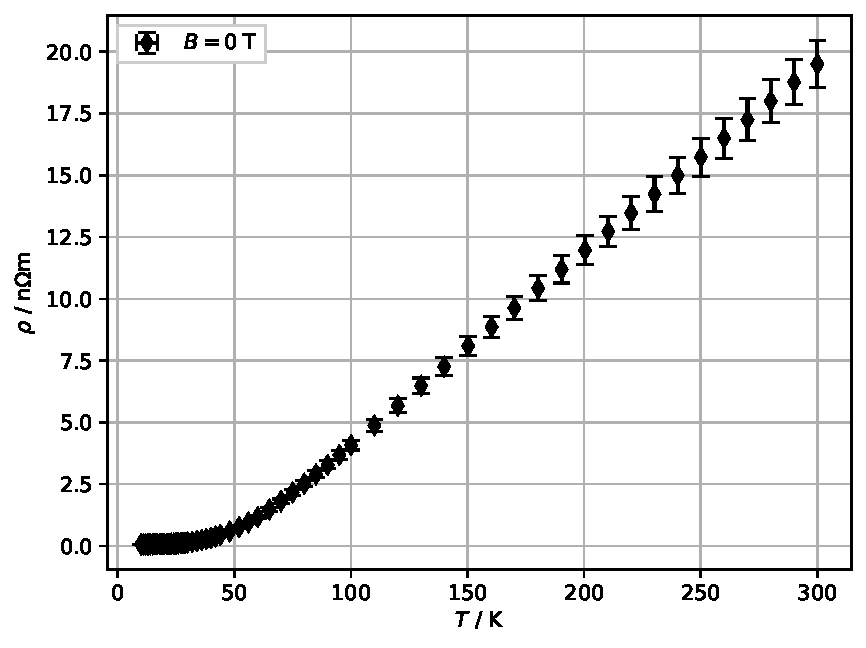
\includegraphics[width=1\textwidth]{../images/resistivity0.pdf}
	\caption{Electric resistivity for different temperatures at zero-field.}\label{fig:res0}
\end{figure}
\begin{figure}
	\centering
	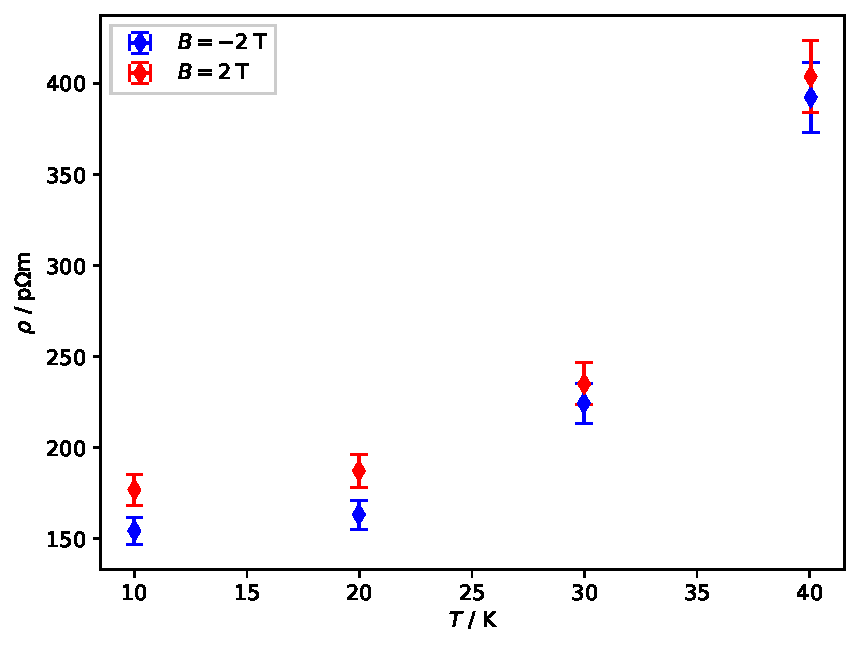
\includegraphics[width=1\textwidth]{../images/resistivity1.pdf}
  \caption{Electric resistivity for different temperatures in a magnetic field at $\SI{2}{T}$ and $\SI{-2}{T}$.}\label{fig:res1}
\end{figure}
\begin{figure}
	\centering
	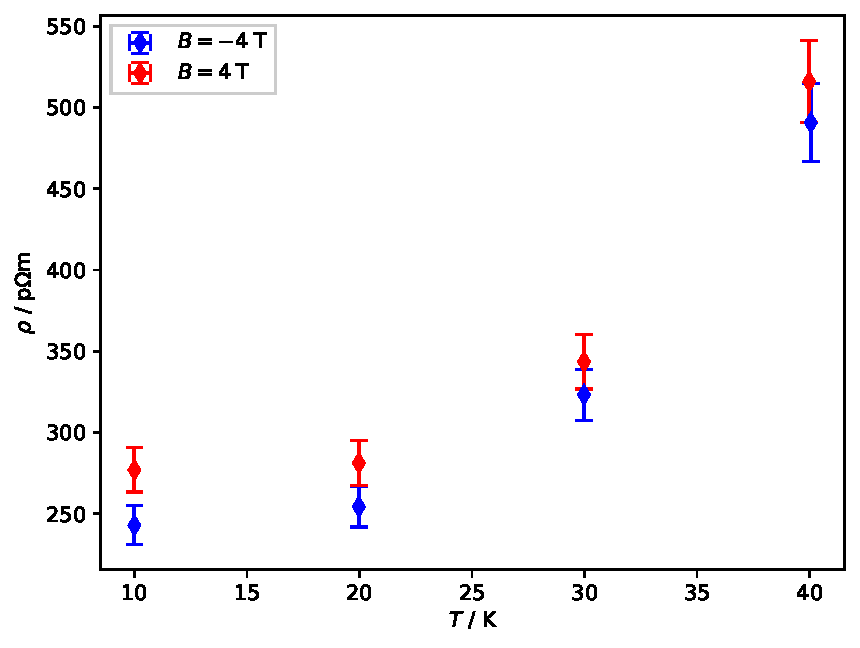
\includegraphics[width=1\textwidth]{../images/resistivity2.pdf}
	\caption{Electric resistivity for different temperatures in a magnetic field at $\SI{4}{T}$ and $\SI{-4}{T}$.}\label{fig:res2}
\end{figure}
\begin{figure}
	\centering
	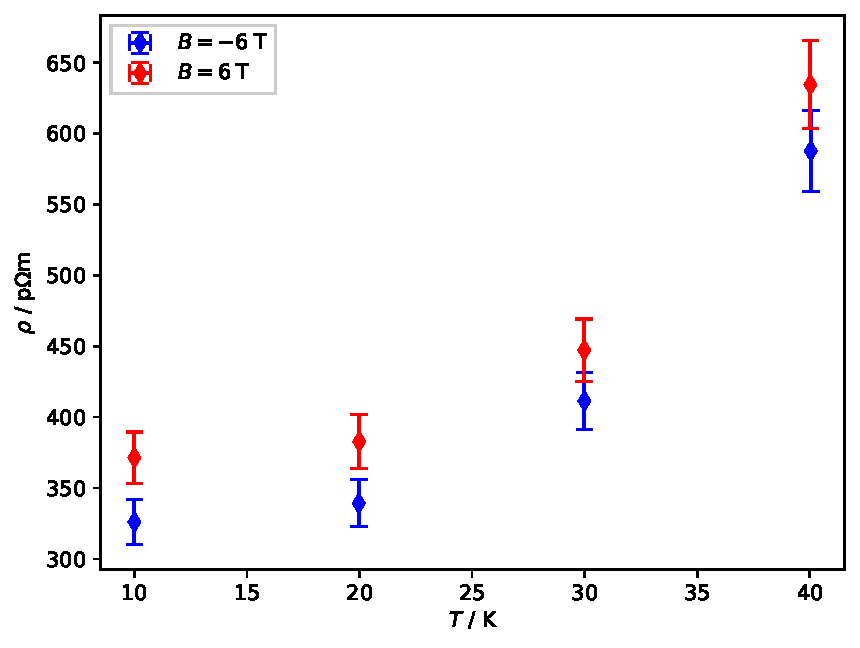
\includegraphics[width=1\textwidth]{../images/resistivity3.pdf}
	\caption{Electric resistivity for different temperatures in a magnetic field at $\SI{6}{T}$ and $\SI{-6}{T}$.}\label{fig:res3}
\end{figure}
The voltages are recorded for different current polarities. They are indicated with $(+)\hat{=}\SI{1}{A}$ and $(-)\hat{=}\SI{-1}{A}$. As can be seen, the calculated resistivity is different for $B$ and $-B$ and for $(+)$ and $(-)$. In the case of the magnetic field, the difference comes from the fact, that the probing contacts are not perfectly centered and the magnetic field induces the hall voltage, which thus contaminates the measured voltage and produces an asymmetry in the measurement. In the case of the different polarities, the difference originates from a residue current, which induces a permanent voltage. In the following analysis, if not shown both, magnetic field and polarity, the average has been takes over the respectively not shown quantity. This cancels the asymmetry:
\begin{align*}
	V_\text{corrected}(B) & = \frac{V(+B)+V(-B)}{2}\\
                        & = \frac{V(+B_0)+V(B_\text{res})+V(-B)-V(B_\text{res})}{2}\\
                        & = \frac{V(+B_0)+V(-B_0)}{2}
\end{align*}

For high temperatures the and at zero-field, the resistivity is linear as shown in \Cref{fig:res_ht}.
\begin{figure}
	\centering
	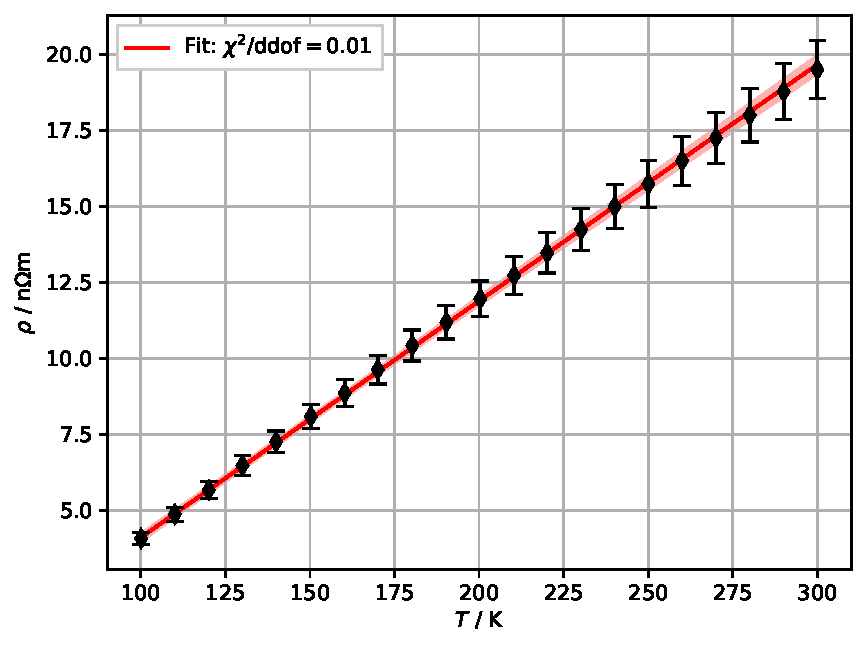
\includegraphics[width=1\textwidth]{../images/resistivity_ht.pdf}
  \caption{Resistivity for hight temperatures at zero-field.Fit: $\rho(T)=\SI{77.8+-1.8}{f\Omega m}+\SI{-3.66+-0.28}{\frac{n\Omega m}{T}}\cdot T$}\label{fig:res_ht}
\end{figure}
The low quality of $\chi^2/\text{ddof}=\SI{0.01}{}$ is due to the large uncertainties. They mainly come from the uncertainty of the geometry, like cross-sectional are and length.
I
To determine the residual resistivity ration (RRR), the resistivity at \SI{300}{K} is devided by the resistivity at \SI{0}{K} in zero-field. Since the lowest resistivity is for \SI{10}{K}, a fit is done with a displaced power law $\rho(T)=\SI{66.59+-0.93}{f\Omega m}+\SI{2.81+-0.079e-18}{\frac{\Omega m}{K^5}}\cdot T^5$.
\begin{figure}
	\centering
	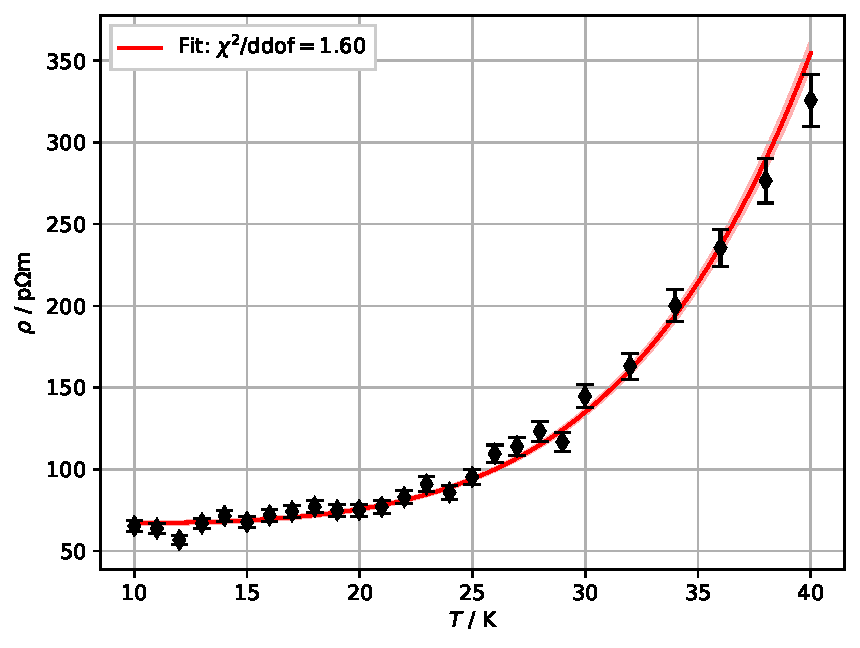
\includegraphics[width=1\textwidth]{../images/resistivity_lt.pdf}
	\caption{Resistivity for low temperatures at zero-field. Fit: $\rho(T)=\SI{66.59+-0.93}{f\Omega m}+\SI{2.81+-0.079e-18}{\frac{\Omega m}{K^5}}\cdot T^5$.}\label{fig:res_lt}
\end{figure}
As a result a RRR of \SI{293\pm14}{} is obtained. As the application is at cryogenic temperatures, this copper should be comparable for OFHC copper, which usually used in this case. A RRR for normal OFHC Copper ranges from 50 to 75 \cite{rrr}. Thus this copper is unusual pure for probably being OFHC copper.

The residual resistivity $\rho(T=\SI{0}{K})$ is now subtracted and plotted in \Cref{fig:rrr}.
\begin{figure}
	\centering
	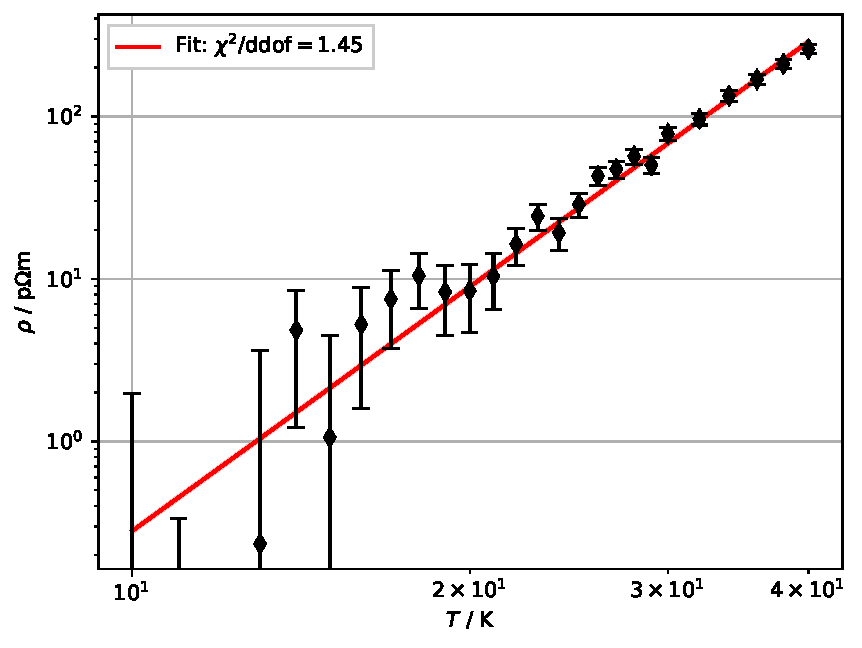
\includegraphics[width=1\textwidth]{../images/resistivity_rrr.pdf}
	\caption{at zero-field}\label{fig:rrr}
\end{figure}
It can be seen that the power law of $T^5$ can model the behaviour very well for low temperatures. The quality of $\chi^2/\text{ddof}=\num{1.54}$ is close to 1, so the model works and the uncertainties are appropriate.

Now instead of plotting for different magnetic fields, the data is plotted for different temperatures. The result is seen in \Crefrange{fig:resT0}{fig:resT3}.
\begin{figure}
	\centering
	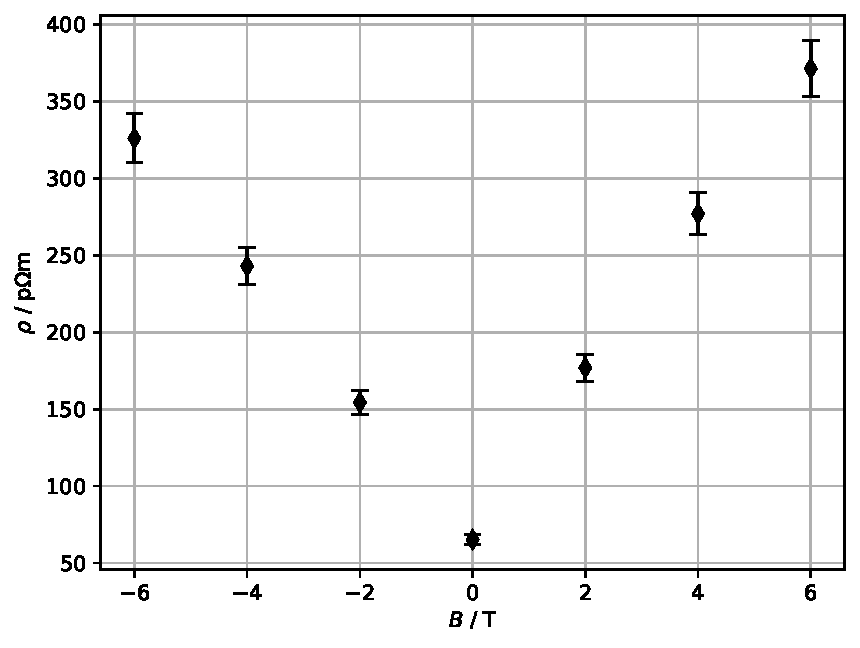
\includegraphics[width=1\textwidth]{../images/resistivity_T0.pdf}
  \caption{Electric resistivity for different magnetic fields at $\SI{10}{K}$}\label{fig:resT0}
\end{figure}
\begin{figure}
	\centering
	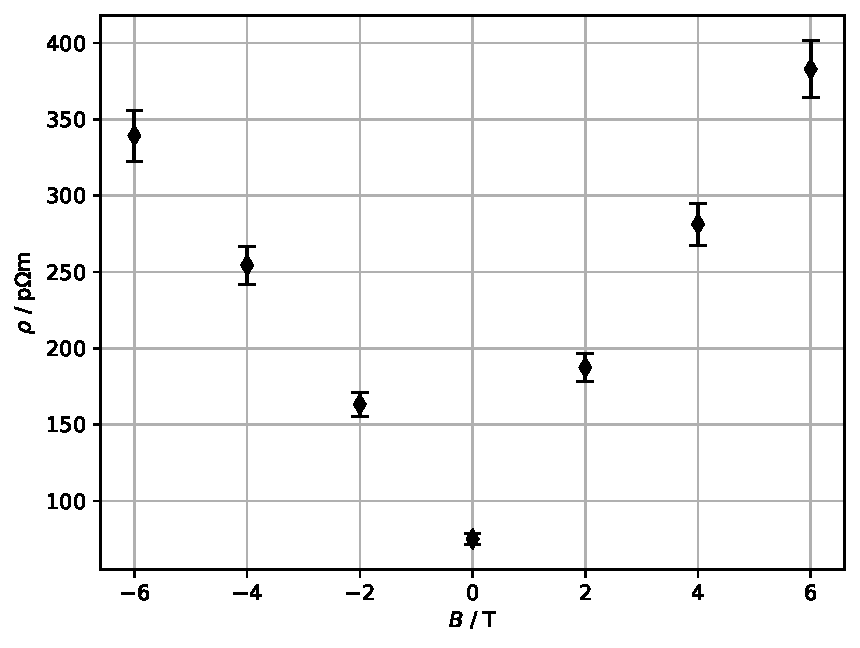
\includegraphics[width=1\textwidth]{../images/resistivity_T1.pdf}
  \caption{Electric resistivity for different magnetic fields at $\SI{20}{K}$.}\label{fig:resT1}
\end{figure}
\begin{figure}
	\centering
	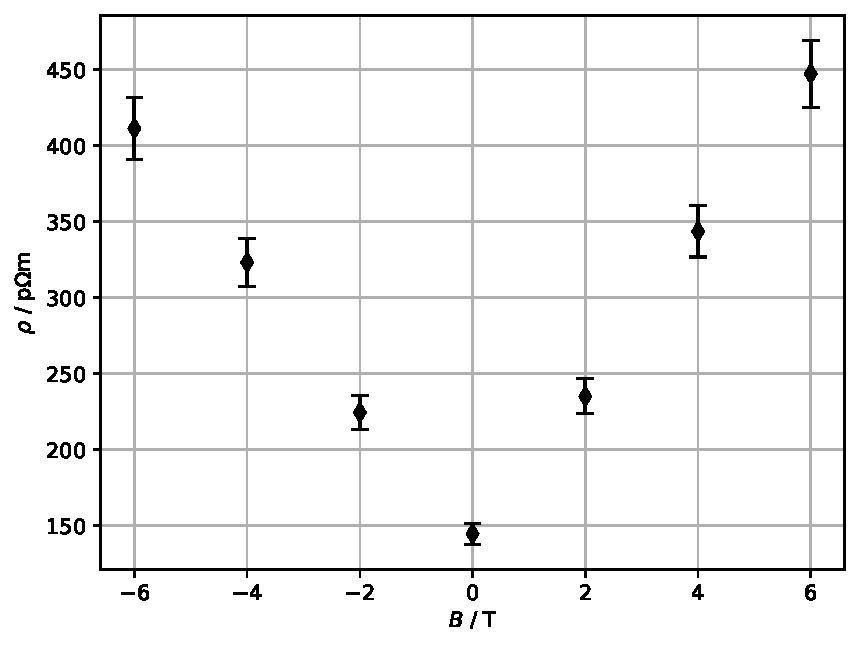
\includegraphics[width=1\textwidth]{../images/resistivity_T2.pdf}
	\caption{Electric resistivity for different magnetic fields at $\SI{30}{K}$.}\label{fig:resT2}
\end{figure}
\begin{figure}
	\centering
	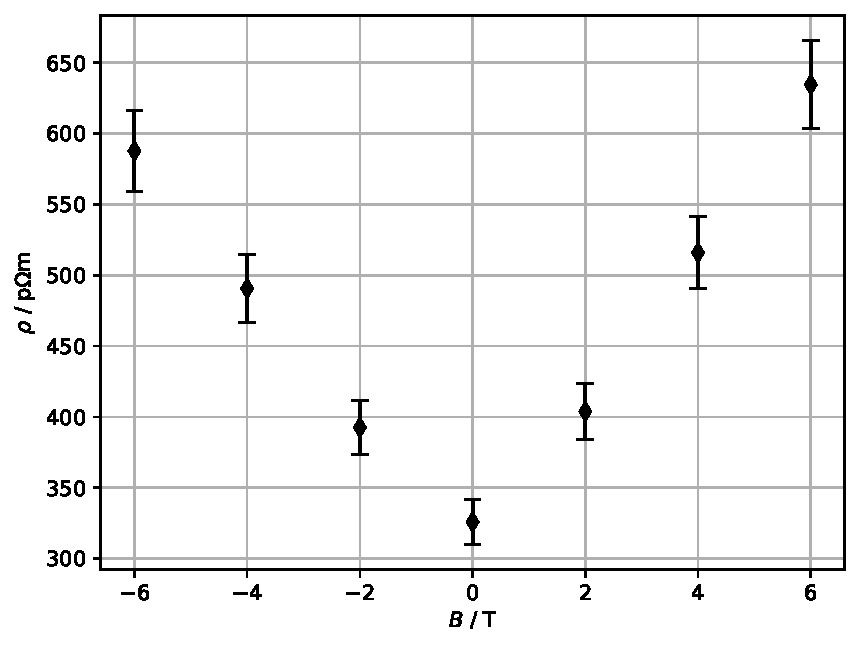
\includegraphics[width=1\textwidth]{../images/resistivity_T3.pdf}
	\caption{Electric resistivity for different magnetic fields at $\SI{40}{K}$.}\label{fig:resT3}
\end{figure}
It can been that the resistivity has no preference for the direction of the magnetic field, except for the hall voltage contamination, and is thus symmetric. Rather strongly prominent is the difference for different current directions, showing that a non-neglectable residue current is present.

Lastly the data can be presented in the Kohler plot. Here the relation
\begin{align}
  \frac{\Delta\rho}{\rho_0}=F\left(\frac{B}{\rho}\right)
\end{align}
with $\Delta\rho=\rho-\rho_0$ and $\rho_0=\rho(T=\SI{0}{K})$ is used. $\rho_0$ is also sometimes defined with $\rho(T=\SI{4.2}{K})$ but since we need to extrapolate in either way, since we only have resistivities for as low as \SI{10}{K}, we use the resistivity at \SI{10}{K}. The Kohler rule says, that relation is independent of the temperature. As seen in \Cref{fig:kohler}, this relation holds.
\begin{figure}
	\centering
	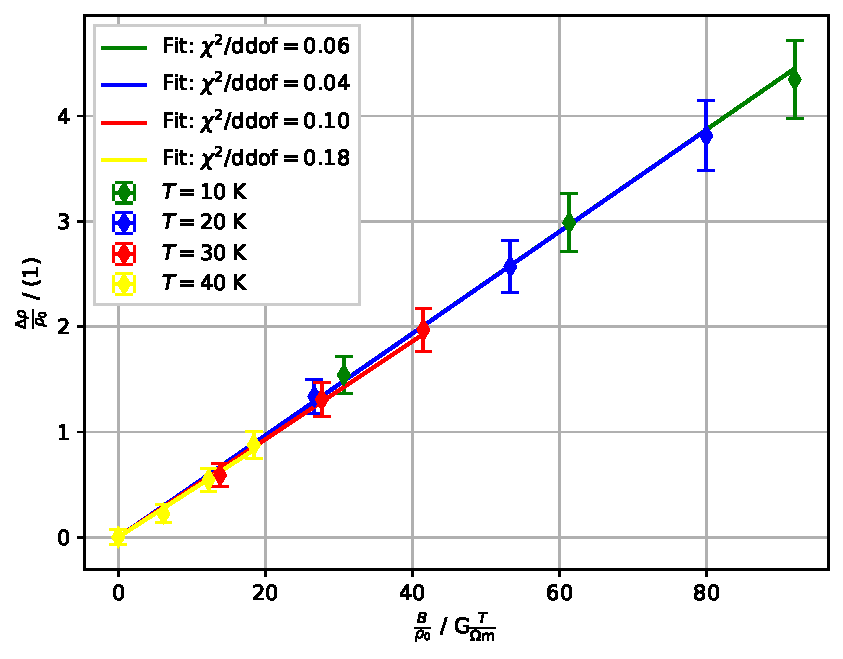
\includegraphics[width=1\textwidth]{../images/Kohler.pdf}
  \caption{Kohler plot with $F(\SI{10}{K})=\SI{48.4+-2.7}{\frac{f\Omega m}{T}}$, $F(\SI{10}{K})=\SI{48.4+-2.8}{\frac{f\Omega m}{T}}$, $F(\SI{10}{K})=\SI{46.5+-3.4}{\frac{f\Omega m}{T}}$ and $F(\SI{10}{K})=\SI{44.9+-5.1}{\frac{f\Omega m}{T}}$.}\label{fig:kohler}
\end{figure}
The function $F$ is material dependent and, taking an weighted average over all temperatures, can be determined to be \SI{46.7\pm 1.6}{\frac{\Omega m}{T}}. All fit-qualities are far below 1, so the uncertainties are overestimated.

\noindent
\begin{tabular}{|p{0.20 \textwidth}|p{0.20 \textwidth}||p{0.20 \textwidth}|p{0.20 \textwidth}|}
\hline
\multicolumn{4}{|c|}{Thermal conductivity at ambient pressure.}\\
\hline
mA&µV&mA&µV\\
\hline
$\num{0.0\pm 0.0}$&$\num{-0.02\pm 0.076}$&$\num{3.0\pm 0.0}$&$\num{35.951\pm 0.086}$\\
$\num{1.0\pm 0.0}$&$\num{4.35\pm 0.12}$&$\num{4.0\pm 0.0}$&$\num{61.75\pm 0.1}$\\
$\num{2.0\pm 0.0}$&$\num{16.28\pm 0.12}$&$\num{5.0\pm 0.0}$&$\num{92.75\pm 0.12}$\\
\hline
\end{tabular}
\begin{tabular}{|p{0.20 \textwidth}|p{0.20 \textwidth}||p{0.20 \textwidth}|p{0.20 \textwidth}|}
\hline
\multicolumn{4}{|c|}{Thermal conductivity in vacuum.}\\
\hline
mA&µV&mA&µV\\
\hline
$\num{0.0\pm 0.0}$&$\num{0.04\pm 0.11}$&$\num{3.0\pm 0.0}$&$\num{39.017\pm 0.083}$\\
$\num{1.0\pm 0.0}$&$\num{4.961\pm 0.07}$&$\num{4.0\pm 0.0}$&$\num{74.75\pm 0.095}$\\
$\num{2.0\pm 0.0}$&$\num{18.784\pm 0.071}$&$\num{5.0\pm 0.0}$&$\num{117.052\pm 0.082}$\\
\hline
\end{tabular}
\begin{tabular}{|p{0.20 \textwidth}|p{0.20 \textwidth}||p{0.20 \textwidth}|p{0.20 \textwidth}|}
\hline
\multicolumn{4}{|c|}{Electric resistivity measurement at ambient pressure.}\\
\hline
mA&µV&mA&µV\\
\hline
$\num{-100.0\pm 0.0}$&$\num{-52.24\pm 0.063}$&$\num{20.0\pm 0.0}$&$\num{11.602\pm 0.061}$\\
$\num{-80.0\pm 0.0}$&$\num{-41.617\pm 0.08}$&$\num{40.0\pm 0.0}$&$\num{22.218\pm 0.077}$\\
$\num{-60.0\pm 0.0}$&$\num{-30.942\pm 0.078}$&$\num{60.0\pm 0.0}$&$\num{32.814\pm 0.079}$\\
$\num{-40.0\pm 0.0}$&$\num{-20.267\pm 0.078}$&$\num{80.0\pm 0.0}$&$\num{43.417\pm 0.082}$\\
$\num{-20.0\pm 0.0}$&$\num{-9.615\pm 0.08}$&$\num{100.0\pm 0.0}$&$\num{54.094\pm 0.07}$\\
$\num{0.0\pm 0.0}$&$\num{0.765\pm 0.071}$&&\\
\hline
\end{tabular}
\begin{tabular}{|p{0.20 \textwidth}|p{0.20 \textwidth}||p{0.20 \textwidth}|p{0.20 \textwidth}|}
\hline
\multicolumn{4}{|c|}{Electric resistivity measurement in vacuum.}\\
\hline
mA&µV&mA&µV\\
\hline
$\num{-100.0\pm 0.0}$&$\num{-52.344\pm 0.074}$&$\num{20.0\pm 0.0}$&$\num{11.29\pm 0.085}$\\
$\num{-80.0\pm 0.0}$&$\num{-41.755\pm 0.079}$&$\num{40.0\pm 0.0}$&$\num{21.955\pm 0.081}$\\
$\num{-60.0\pm 0.0}$&$\num{-31.162\pm 0.071}$&$\num{60.0\pm 0.0}$&$\num{32.589\pm 0.089}$\\
$\num{-40.0\pm 0.0}$&$\num{-20.553\pm 0.096}$&$\num{80.0\pm 0.0}$&$\num{43.2\pm 0.082}$\\
$\num{-20.0\pm 0.0}$&$\num{-9.963\pm 0.079}$&$\num{100.0\pm 0.0}$&$\num{53.895\pm 0.084}$\\
$\num{0.0\pm 0.0}$&$\num{0.633\pm 0.081}$&&\\
\hline
\end{tabular}

\bibliography{refs}
\end{document}
